\documentclass[../main.tex]{subfiles}

\begin{document}

\section{Conjuntos}
\subsection{¿Qué es un conjunto?}
Un conjunto corresponde a una colección bien definida de objetos. Estos objetos son denominados como \textbf{elementos del conjunto} y se dice que estos \textbf{pertenecen} (expresado con el simbolo $\in$) a él.\\
Cuando definimos un conjunto, se usan símbolos de llaves y dentro se colocan todos los objetos que pertenecen al conjunto.\\
Ejemplo:
\[ S = \{ 1, 2, 3, 4 \} \]

\subsection{Nociones básicas de los conjuntos}
\subsubsection{Pertenencia ($\in$)}
Si tenemos un conjunto $S$ y un objeto $a$, se dice que
\begin{itemize}
    \item $a \in S$ cuando el objeto $a$ se encuentra dentro del conjunto S.
    \item $a \not\in S$ cuando el objeto $a$ \textbf{no} se encuentra dentro del conjunto S.
\end{itemize}
\textbf{NOTA:} Un objeto puede ser un conjunto. Esto significa que un conjunto puede pertenecer a otro conjunto.

\subsubsection{Subconjunto ($\subseteq$)}
Considerando a un conjunto $A$ y un conjunto $B$, se dice que $A$ es subconjunto de $B$ si
\[ \forall x . x \in A \rightarrow x \in B \]
En otras palabras, $A$ es subconjunto de $B$ si todo elemento presente en $A$ está presente en $B$ también. Cuando esto ocurre, se denota como $A \subseteq B$ (y cuando no, lógicamente se escribe como $A \not\subseteq B$)

\subsubsection{Igualdad de conjuntos}
Diremos que dos conjuntos $A$ y $B$ son iguales si se cumple que
\[ A \subseteq B \wedge B \subseteq A \quad \text{o, escrito de otra forma} \quad \forall x . x \in A \leftrightarrow x \in B \]
En palabras simples, dos conjuntos son iguales cuando ambos conjuntos tienen exactamente los mismos objetos, sin ninguno que pertenezca a un conjunto y no a otro. Esto se expresa como $A = B$ (y cuando no, $A \not= B$).

\subsubsection{Conjunto vacío}
Existe un conjunto único $\emptyset$, el cual llamamos \textit{conjunto vacío}, el cual cumple que 
\[ \forall x . x \not\in \emptyset \]

\subsection{Descripción de un conjunto}
\begin{enumerate}
    \item Por extensión: Este es el método más básico y el cual se describió anteriormente. Simplemente se listan todos los contenidos del conjunto entre llaves.\\
    Ejemplo: \[ S = \{ 1, 2, 3, 4 \} \]
    \item Por comprensión: Se define una propiedad $\delta(x)$ en algún lenguaje formal que solo cumplen los elementos del conjunto.\\
    Ejemplo: \[ S = \{ x | \delta(x) \text{ es verdadero} \} \]
    Ejemplo un poco más creativo: \[ P = \{ x | \forall x . x \text{ es par} \} \]
\end{enumerate}

\subsection{Paradoja de Russell o Paradoja del Barbero (1901)\footnote{Esta sección contiene información extraída del \href{https://es.wikipedia.org/wiki/Paradoja_de_Russell}{siguiente artículo de Wikipedia}.}}
\begin{wrapfigure}{r}{0.25\textwidth}
    \centering
    
\includegraphics[width = 0.25\textwidth]{b_russell.png}
    \text{B. Russell (1872 - 1970)}
\end{wrapfigure}
Esta es una paradoja enunciada por Bertrand Russell. Para comenzar, se define el siguiente conjunto
\[ S^* = \{ B \  | \  B \not\in B \} \]
$S^*$ corresponde al ``conjunto de todos los conjuntos que no se contienen a si mismos como miembros''. Ahora, recordemos que por la definición de lo que es un conjunto, esto es equivalente a
\[ \forall B . B \in S^* \leftrightarrow B \not\in B \]
O sea, ``cada conjunto es elemento de $B$ si y solo si no es elemento de si mismo''. Debido a que $B$ es un conjunto, lo podemos sustituir de la siguiente forma
\[ S^* \in S^* \leftrightarrow S^* \not\in S^* \]
lo cual es una contradicción.\\
Esto puede ser un poco complicado de entender así. Intentemos entenderlo con la historia del Barbero.

\includegraphics[width = 0.5\textwidth]{barb_1.png}
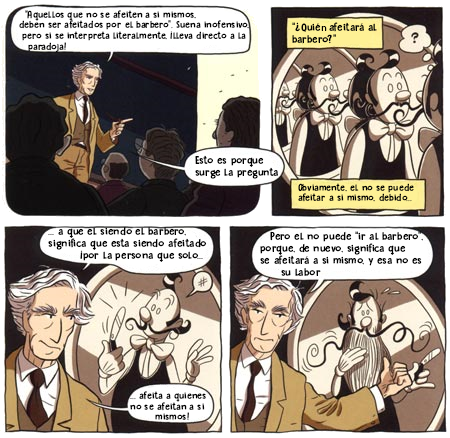
\includegraphics[width = 0.5\textwidth]{barb_2.png}

Una definición como esta es bastante problemática. El problema aquí es \textit{``considerar definiciones que se referencian a si mismas''}. Esto nos deja de lección que no todas las definiciones son válidas en la teoría de conjuntos.\footnote{Todas las definiciones que se verán durante el curso son válidas, pero esto es una lección de que no siempre es así.}

\subsection{Operaciones sobre conjuntos}
\begin{itemize}
    \item Unión ($\cup$): $A \cup B$ son todos los elementos que se encuentran en $A$ o en $B$.
    \[ A \cup B = \{ x | x \in A \vee x \in B \} \]
    \item Intersección ($\cap$): $A \cap B$ son todos los elementos que se encuentran en $A$ y $B$ al mismo tiempo.
    \[ A \cap B = \{ x | x \in A \wedge x \in B \} \]
    \item Diferencia ($\backslash$): $A \backslash B$ son todos los elementos que se encuentran en $A$ y no en $B$.
    \[ A \backslash B = \{ x | x \in A \wedge x \not\in B \} \]
    \item Complemento ($A^C$): $A^C$ corresponde a todos los elementos que no se encuentran en $A$.
    \[ A^C = \{ x | x \not\in A\} \]
\end{itemize}

\subsubsection{Propiedades de las operaciones sobre conjuntos}
Para conjuntos $A$, $B$ y $C$ y un universo $\mathcal{U}$ tenemos las siguientes propiedades
\begin{enumerate}
    \item Asociatividad:
    \[
        \begin{tabular}{rcl}
            $A \cup (B \cup C)$ & $=$ & $(A \cup B) \cup C$ \\
            $A \cap (B \cap C)$ & $=$ & $(A \cap B) \cap C$ \\
        \end{tabular}
    \]
    \item Conmutatividad:
    \[
        \begin{tabular}{rcl}
            $A \cup B$ & $=$ & $B \cup A$ \\
            $A \cap B$ & $=$ & $B \cap A$ \\
        \end{tabular}
    \]
    \item Idempotencia:
    \[
        \begin{tabular}{rcl}
            $A \cup A$ & $=$ & $A$ \\
            $A \cap A$ & $=$ & $A$ \\
        \end{tabular}
    \]
    \item Absorción:
    \[
        \begin{tabular}{rcl}
            $A \cup (A \cap B)$ & $=$ & $A$ \\
            $A \cap (A \cup B)$ & $=$ & $A$ \\
        \end{tabular}
    \]
    \item Distributividad:
    \[
        \begin{tabular}{rcl}
            $A \cup (B \cap C)$ & $=$ & $(A \cup B) \cap (A \cup C)$ \\
            $A \cap (B \cup C)$ & $=$ & $(A \cap B) \cup (A \cap C)$ \\
        \end{tabular}
    \]
    \item De Morgan
    \[
        \begin{tabular}{rcl}
            $(A \cup B)^C$ & $=$ & $A^C \cap B^C$ \\
            $(A \cap B)^C$ & $=$ & $A^C \cup B^C$ \\
        \end{tabular}
    \]
    \item Elemento neutro:
    \[
        \begin{tabular}{rcl}
            $A \cup \emptyset$ & $=$ & $A$ \\
            $A \cap \mathcal{U}$ & $=$ & $A$ \\
        \end{tabular}
    \]
    \item Dominación:
    \[
        \begin{tabular}{rcl}
            $A \cap \emptyset$ & $=$ & $\emptyset$ \\
            $A \cup \mathcal{U}$ & $=$ & $\mathcal{U}$ \\
        \end{tabular}
    \]
    \item Elemento inverso:
    \[
        \begin{tabular}{rcl}
            $A \cup A^C$ & $=$ & $\mathcal{U}$ \\
            $A \cap A^C$ & $=$ & $\emptyset$ \\
        \end{tabular}
    \]
\end{enumerate}

\subsubsection{Paréntesis y precedencia}
Se asumirá el siguiente orden de precedencia entre operadores
\[
    \begin{tabular}{cc}
        Operadores & Precedencia \\ \hline
        $.^C$ & $1$ \\
        $\cap$ & $2$ \\
        $\cup$ & $3$
        
    \end{tabular}
\]

\subsubsection{Operaciones generalizadas}
\begin{itemize}
    \item Unión generalizada: $\bigcup \mathcal{S}$ son todos los elementos que pertenecen a algún elemento de $\mathcal{S}$.
    \[ \bigcup \mathcal{S} = \{ x \  | \ \exists A .\  A \in \mathcal{S} \wedge x \in A \} = \bigcup_{A \in \mathcal{S}} A = \bigcup_{i = 1}^{k} A_i \]
    \item Intersección generalizada: $\bigcap \mathcal{S}$ son todos los elementos que pertenecen a todos los elementos de $\mathcal{S}$
    \[ \bigcap \mathcal{S} = \{ x \  | \ \forall A .\  A \in \mathcal{S} \rightarrow x \in A \} = \bigcap_{A \in \mathcal{S}} A = \bigcap_{i = 1}^{k} A_i \]
\end{itemize}


\end{document}